\documentclass[tikz,border=5pt]{standalone}
\usepackage{luatexja}
\usepackage[hiragino-pron]{luatexja-preset}
\usepackage{amsmath,amssymb}
\usepackage{pgfplots}
\pgfplotsset{compat=1.18}
\usetikzlibrary{arrows.meta,calc,decorations.markings,patterns,positioning}

% Common styles
\tikzset{
  axis/.style={-{Stealth[length=6pt]}, thick},
  curve/.style={thick, red},
  dashed curve/.style={thick, dashed, blue},
  dot/.style={circle, fill, inner sep=1.5pt},
  open dot/.style={circle, draw, fill=white, inner sep=1.5pt},
}

\begin{document}
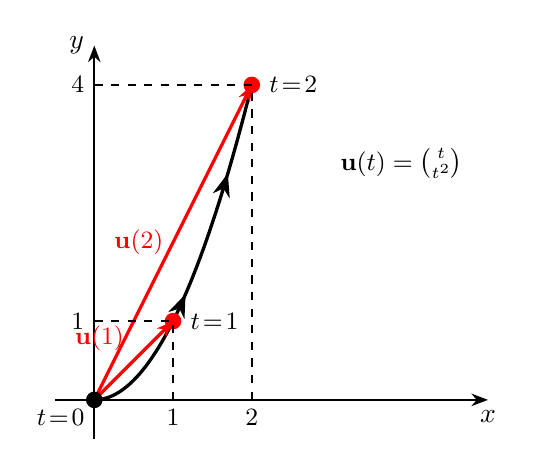
\begin{tikzpicture}
  % Axes
  \draw[axis] (-0.5,0) -- (5,0) node[below] {$x$};
  \draw[axis] (0,-0.5) -- (0,4.5) node[left] {$y$};

  % Trajectory: (t, t^2) for t from 0 to 2
  \draw[very thick, domain=0:2, samples=50,
    decoration={markings,
      mark=at position 0.4 with {\arrow{Stealth}},
      mark=at position 0.75 with {\arrow{Stealth}}
    }, postaction={decorate}]
    plot (\x, {\x*\x});

  % Vector from origin to t=1
  \draw[-{Stealth[length=6pt]}, red, very thick] (0,0) -- (1,1);
  \node[red, above left, font=\small] at (0.5,0.5) {$\mathbf{u}(1)$};

  % Vector from origin to t=2
  \draw[-{Stealth[length=6pt]}, red, very thick] (0,0) -- (2,4);
  \node[red, left, font=\small] at (1,2) {$\mathbf{u}(2)$};

  % Points
  \fill (0,0) circle (3pt);
  \node[below left, font=\small] at (0,0) {$t\!=\!0$};

  \fill[red] (1,1) circle (3pt);
  \node[right, font=\small] at (1.1,1) {$t\!=\!1$};

  \fill[red] (2,4) circle (3pt);
  \node[right, font=\small] at (2.1,4) {$t\!=\!2$};

  % Dashed lines for t=2
  \draw[dashed, semithick] (2,0) node[below, font=\small] {$2$} -- (2,4);
  \draw[dashed, semithick] (0,4) node[left, font=\small] {$4$} -- (2,4);

  % Dashed lines for t=1
  \draw[dashed, semithick] (1,0) node[below, font=\small] {$1$} -- (1,1);
  \draw[dashed, semithick] (0,1) node[left, font=\small] {$1$} -- (1,1);

  % Label
  \node[right, font=\small] at (3,3) {$\mathbf{u}(t) = \binom{t}{t^2}$};
\end{tikzpicture}
\end{document}
